\documentclass[../main]{subfiles}
\begin{document}
\chapter{概率基础}

\begin{introduction}
    \item 事件
    \item 古典概型与几何概率
    \item 条件概率与独立
    \item 乘法法则
    \item 全概率公式
    \item Bayes法则
\end{introduction}

\section{概率空间}

\begin{definition}[样本空间]
    随机试验可能出现的结果称为\textbf{样本点}(sample point),用$\omega$表示。样本的全体构成\textbf{样本空间}(sample space),用$\Omega$表示。
\end{definition}

\begin{definition}[事件的古典定义]
    样本点$\omega$的集合称为\textbf{事件}(event)。
\end{definition}

我们关心的随机现象被抽象为集合, 逻辑运算(且, 或, 非, etc.)对应成集合论运算(交, 并, 补, etc.)。

\begin{property}
    集合的运算性质:
    \begin{description}
        \item [交换律] $A \cup B = B \cup A, \quad AB = BA$
        \item [结合律] $(A \cup B) \cup C = A \cup (B \cup C), (AB)C = A(BC)$
        \item [分配律]
              \begin{gather}
                  (A \cup B) \cup C = A \cup (B \cup C),\\
                  (A \cap B) \cup C = (A \cup C) \cap (B \cup C).
              \end{gather}
        \item [对偶律(De Morgan's laws)]
              \begin{gather}
                  \text{事件并的对立等于对立的交:} \quad \overline{A \cup B} = \overline{A} \cap \overline{B},\\
                  \text{事件交的对立等于对立的并:} \quad \overline{A \cap B} = \overline{A} \cup \overline{B}.
              \end{gather}
    \end{description}
\end{property}

为方便概率的定义,并不把$\Omega$的一切子集作为事件,应避免不可测集的出现。

\begin{definition}[事件域]
    事件构成的全体称为\textbf{事件域}$\mathscr{F}$,是$\Omega$的子集族(collection of subsets),应满足\underline{\,$\sigma$代数}的要求:
    \begin{itemize}
        \item $\emptyset \in \mathscr{F}$, 无事发生;
        \item $A\in\mathscr{F} \implies A^{\complement}\in\mathscr{F}$, 即$\mathscr{F}$对补集运算(逻辑上的非)封闭;
        \item $A_{1},\dots,A_{n},\ldots \in \mathscr{F} \implies \bigcap_{n=1}^{\infty}A_{n} \in \mathscr{F}$, 即$\mathscr{F}$对可数交运算(逻辑上的可数多个且)封闭.
    \end{itemize}
\end{definition}

\begin{note}
    可数性是为了在数学上能够恰当地处理\underline{无穷}的概念, 术语中的$\sigma$指的就是\underline{可数并}。由对偶原理可得$\sigma$域同时对可数并运算封闭. 即$\sigma$域对逆, 并, 交, 差的可数次运算封闭.
\end{note}

事件域根据问题的不同要求适当选取, 在概率定义没有困难时, 应尽量选大, 通常以$\Omega$的一切子集作为事件域. 当$\Omega$给定后,若某些子集必须作为事件处理, 能否找到包含他们的$\sigma$域?

\begin{proposition}
    若给定$\Omega$的一个非空集族$\mathscr{G}$, 必存在$\Omega$上唯一的$\sigma$域$\mathfrak{m}(\mathscr{G})$, 满足下列性质:
    \begin{itemize}
        \item 包含$\mathscr{G}$
        \item 若其他$\sigma$域包含$\mathscr{G}$, 则必包含$\mathfrak{m}(\mathscr{G})$
    \end{itemize}
    这个$\mathfrak{m}(\mathscr{G})$称为包含$\mathscr{G}$的最小$\sigma$域, 或由$\mathscr{G}$扩张而成的$\sigma$域.
\end{proposition}

\emph{扩张}, 或者称为\emph{延拓}, 是数学中很重要的一个概念, 大抵是将某映射的定义域适当扩大, 不改变在初始定义域上的映射取值(注意值域可能是比较抽象的集合, 配备了某些操作之后被称为空间), 同时在扩大后的定义域上仍然保持某些优良的性质. 与此相对的概念是\emph{限制}, 即关心局部上可能更加漂亮的性质, 把初始的定义域适当缩小.

\begin{proof}
    由于$\Sigma$的一切子集构成的集类包含$\mathscr{G}$, 所以$\mathfrak{m}$存在. 再取$\Sigma$上满足此条件的$\sigma$域之交作为$\mathfrak{m}(\mathscr{G})$即可.
\end{proof}

特别地, 实数集$\R$的子集族$\{(-\infty,x] : x\in\R\}$生成的$\sigma$代数$\mathscr{B}_{\R}$称为$\R$上的\emph{Borel代数}.

\begin{definition}[Borel集]
    设$\mathbb{R}^1$为全集, 形为$[a,b)$构成的集类产生的$\sigma$域称为\textbf{一维Borel$\sigma$域}, 记为$\mathscr{B}_1$, 其中的元素称为\textbf{一维Borel集}
\end{definition}

若$x,y$为任意实数,由于:
\begin{align*}
    \{x\}  & =  \bigcap_{n=1}^{\infty}\left[x, x+\frac{1}{n}\right) \\
    (x, y) & =  [x, y)-\{x\}                                        \\
    [x, y] & =  [x, y)+\{y\}                                        \\
    (x, y] & =  [x, y)+\{y\}-\{x\}
\end{align*}
因此$\mathscr{B}_1$包含一切开区间, 闭区间, 单个实数, 可列个实数, 以及他们经可列次逆, 并, 交, 差运算的集合.

\begin{definition}[概率空间]
    定义在\underline{事件域}(非样本空间)上的集合函数$P : \mathscr{F} \to \mathbb{R}$称为\textbf{概率}的条件是:
    \begin{description}
        \item[非负性] $P(A)\ge 0 , \forall A \in \mathscr{F}$
        \item[规范性] $P(\Omega) = 1$; (如果没有这条就是一般的{\color{lightgray}有限}\emph{测度})
        \item[可列可加性] 若$A_{1},\dots,A_{n},\ldots \in \mathscr{F}$两两不交, 即$A_{i}\cap A_{j} = \emptyset, \ \forall i\neq j$, 则$P(\bigcup_{n=1}^{\infty}A_{n}) = \sum_{n=1}^{\infty}P(A_{n})$.
    \end{description}
    我们称$(\Omega,\mathscr{F},P)$为一个\textbf{概率空间}(probability space)
\end{definition}

\begin{property}
    概率的性质:
    \begin{itemize}
        \item $P(\Omega)=1$;
        \item $P(A^{\complement})=1-P(A)$;
        \item 若$A \subseteq B $ 则 $P(A)\le P(B)$;
    \end{itemize}
\end{property}

\begin{corollary}[加法公式]
    基础形式:
    \[ P(A \cup B) = P(A) + P(B) - P(AB) \]
    一般形式:
    \begin{align*}
         & P\left(A_{1} \cup A_{2} \cup \cdots \cup A_{n}\right) =  \sum_{i=1, \cdots, n} P\left(A_{i}\right)-\sum_{\substack{i<j \\
        i, j=1, \cdots, n}} P\left(A_{i} A_{j}\right)                                                                             \\
         & +\sum_{\substack{i<j<k                                                                                                 \\i, j, k=1, \cdots, n}} P\left(A_{i} A_{j} A_{k}\right)-\cdots+(-1)^{n-1} P\left(A_{1} A_{2} \cdots A_{n}\right)
    \end{align*}
    特别地, 若事件出现个数相同时概率相等,则可简化为:
    \[ P\left(A_{1} \cup A_{2} \cup \cdots \cup A_{n}\right)=n P_{1} - \binom{n}{2} P_{2} + \binom{n}{3} P_{3}- \cdots+(-1)^{n-1} P_{n} \]
\end{corollary}

显然,可列可加性可以推出有限可加性. 但是一般来讲,由有限可加性并不能推出可列可加性. 设$A_i \in \mathscr{F}, i=1,2,\cdots $且两两互不相容, 若希望由有限可加性推出可列可加性,则需要下式成立:
\[ \lim_{n \to \infty}P(\sum_{i=1}^n A_i) =P(\lim_{n \to \infty}\sum_{i=1}^{n} A_i) \]

\begin{definition}
    对于$\mathscr{F}$上的集合函数$P$,若它对$\mathscr{F}$中任何一个单调不减的集序列$\{ S_n \}$(即$ S_n \in \mathscr{F}, S_n \subseteq  S_{n+1} $)均满足:
    \[ \lim_{n \to \infty}P(S_n) =P(\lim_{n \to \infty} S_n) \]
    则称它是\textbf{下连续的}.
\end{definition}

故若令$S_n = \sum_{i=1}^n A_n$, 则可列可加性条件等价于有限可加性加下连续.

\section{古典概型与几何概率}

\subsection{古典概型}

古典概型的基本思想:
\begin{description}
    \item[有限个样本点] 所涉及的随机现象只有有限个样本点, 譬如为 $n$ 个, 且这些事件是两两互不相容的;
    \item[等可能性] 每个样本点发生的可能性相等
\end{description}

\begin{definition}
    若事件 $A$ 含有 $k$ 个样本点, 则事件 $A$ 的概率为
    \[  P (A) = \frac{\text{事件 } A \text{ 所含样本点的个数}}{\Omega \text{ 中所有样本点的个数}} = \frac{k}{n} \]
\end{definition}

\begin{note}
    事实上,古典概型的大部分问题都能形象化地用摸球模型来描述以后我们经常研究摸球模型,意义即在于此.
\end{note}

\section{条件概率}

\begin{definition}[条件概率]
    令$A,B \in \mathscr{F}$, 且$P(B)>0$称
    \[ P(A|B) = \frac{P(A \cap B)}{P(B)}\]
    为\textbf{基于于$B$的条件概率}(probability conditional on $B$), 这仍然是一个概率测度.
\end{definition}

\begin{theorem}[乘法法则]
    令$A,B \in \mathscr{F}$, 且$P(B)>0$, 则
    \[ P(A \cap B) = P(A|B)P(B) \]
    泛化后有:
    \[ P(A_1 \cap A_2 \cap \cdots \cap A_n) = P(A_{1})P(A_2|A_1)P(A_3|A_1\cap A_2) \cdots  \]
\end{theorem}

\begin{theorem}[全概率公式]
    设 $B_1, B_2, \dotsc, B_n$ 为样本空间 $\Omega$ 的一个分割, 且互不相容, 即$\bigcup _{i=1} ^n B_i = \Omega, B_i B_j= \emptyset for i \neq j $
    如果 $P(B_i) > 0$, $i=1, 2, \dotsc, n$,
    则对任一事件 $A$ 有
    \begin{equation}
        P(A) = \sum_{i=1}^n P(B_i) P(A | B_i).
    \end{equation}
\end{theorem}

\begin{note}
    $P(A | B_i)$可视为事件$A$在$B_i$上的平均, $P(B_i)$则为其权重.
\end{note}

\begin{theorem}[Bayes定理]
    设 $B_1, B_2, \dotsc, B_n$ 为样本空间 $\Omega$ 的一个分割, 且互不相容, 即$\bigcup _{i=1} ^n B_i = \Omega, B_i B_j= \emptyset for i \neq j $
    如果 $P(A) > 0$, $P(B_i) > 0$, $i = 1,2, \dotsc, n$,
    则
    \begin{equation}
        P (B_i | A) = \frac{P(B_i) P(A|B_i)}{\sum_{j=1}^n P(B_j) P(A|B_j)}
    \end{equation}
\end{theorem}

\begin{definition}[事件的独立性]
    如果$A,B\in\mathscr{F}$满足
    \[ P(A\cap B) = P(A)P(B), \]
    则称$A$与$B$\textbf{独立}(independent), 记为$A \Vbar B$.

    对于事件集$A_1, A_2, \dotsc, A_n$, 若对于其中任意子集$A_{i_1}, A_{i_2}, \dotsc, A_{i_n}$有:
    \[ P(A_{i_1} \cap \cdots  \cap A_{i_n}) =P(A_{i_1})\cdots P(A_{i_n})  \]
    则称此事件集\textbf{相互独立}(mutually independent)
\end{definition}

\begin{note}
    当$P(A)>0$时, 我们有$ P(B|A) = P(B) \iff B \Vbar A$, 由此可得到\underline{$B$独立于$A$}的直观理解
\end{note}

\begin{property}
    独立性是对称的, 即$A \Vbar B \iff B \Vbar A$. 若两事件独立, 则其补集也独立.
    \begin{center}
        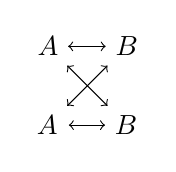
\begin{tikzpicture}
            \node[draw=none,fill=none] (1) at(0,0) {$A^{\complement}$};
            \node[draw=none,fill=none] (2) at(1,0) {$B^{\complement}$};
            \node[draw=none,fill=none] (3) at(0,1) {$A$};
            \node[draw=none,fill=none] (4) at(1,1) {$B$};
            \draw[<->] (1)--(2);
            \draw[<->] (1)--(4);
            \draw[<->] (3)--(2);
            \draw[<->] (3)--(4);
        \end{tikzpicture}
    \end{center}
\end{property}

\begin{definition}[事件域的独立性]
    若$\mathscr{G} \subset \mathscr{F}$与$\mathscr{H} \subset \mathscr{F}$满足
    \[ A \Vbar B, \quad \forall A\in\mathscr{G},\ B\in\mathscr{H}, \]
    则称$\mathscr{G}$与$\mathscr{H}$独立, 记为$\mathscr{G} \Vbar \mathscr{H}$
\end{definition}

测度论告诉我们一个重要结果: 如果$\mathscr{G}$对交集运算封闭, 那么成立$\mathscr{G}\Vbar\mathscr{H} \implies \sigma(\mathscr{G}) \Vbar \mathscr{H}$

\end{document}